%%%%%%%%%%%%%%%%%%%%%%%%%%%%%%%%%%%%%%%%%
\documentclass[a4paper, 11pt, parskip=half]{scrartcl}
\usepackage[english]{babel}
\usepackage{DejaVuSerif}
\usepackage{DejaVuSans}
\usepackage{sourcecodepro}
\usepackage[utf8x]{inputenc}
\usepackage[T1]{fontenc}
\usepackage{amsmath}
\usepackage{graphicx}
\usepackage[colorinlistoftodos]{todonotes}
\usepackage{hyperref}
\usepackage{float}
\usepackage{caption}

%\usepackage{fancyhdr}
%\pagestyle{fancy}

\areaset{17cm}{22.5cm}              % Set page width and height

\begin{document}
\begin{titlepage}
\pagenumbering{gobble}
\newcommand{\HRule}{\rule{\linewidth}{0.1mm}} 
\center % Center everything on the page
 

\textsc{Computer science engineering}\\[0.3cm] % heading course Number
\textsc{\Large Internet Of Things}\\[0.5cm] % heading course name
\textsc{\large Project n°1}\\[0.5cm] % Minor heading


\HRule \\[0.4cm]
{ \huge \bfseries Waste management system}\\[0.1cm] % Title of your Homework/assignment
\HRule \\[1.5cm]
 
%---------------------------------------------------------------------------------
%	AUTHOR SECTION (EDIT THE NAME and T.NO., only)
%---------------------------------------------------------------------------------

\begin{minipage}{0.4\textwidth}
\begin{flushleft} \large

Fabio \textsc{Codiglioni}\\ 919897 - 10484720  % Enter Your name and T.No.
\end{flushleft}
\begin{flushleft} \large


Alessandro \textsc{Nichelini}\\ 949880 - 10497404  % Enter Your name and T.No.
\end{flushleft}


\end{minipage}
\begin{minipage}{0.4\textwidth}

\begin{flushright} \large
\emph{Professor:}\\
Matteo \textsc{Cesana} \\[0.4cm]% Supervisor's Name
\emph{Teaching assistant:} \\
Edoardo Longo
\end{flushright}

\end{minipage}\\[1cm]
{\large Academic year 2018/2019}
\begin{figure}[H]
	\centering
	
\includegraphics[width=\textwidth,height=5.7cm,keepaspectratio]{resources/polimi_logo}% \\[0.5cm] % 
\end{figure}

\vfill % Fill the rest of the page with white-space

\end{titlepage}

\tableofcontents          % Required
\listoffigures
\newpage

\pagenumbering{arabic}

\section{Abstract}
This document describes the implementation of our project for the IoT course.

We decided to implement the project number 1: \textit{Waste management system}. We used Contiki as the operating system for the IoT devices and Cooja as the simulator. We also used Node-RED to make data available to the external world and to build a light dashboard to display the system status and the transmitted messages.

We implemented all requested requirements by writing two different firmwares: one for the bins and one for the truck. We manually set up the requested node layout in Cooja and we randomly generated a second layout.

Full source code is available at our repo: \\
\url{https://github.com/fabiocody/CodiglioniNicheliniIoT}

\section{Implementation design choices}

\subsection{Architecture}

Each one of the two firmwares lives almost exclusively in a single \texttt{.c} source file (except for some utility functions in \texttt{toolkit.c}), and can be summed up by the following figures.

\begin{figure}[H]
	\centering
	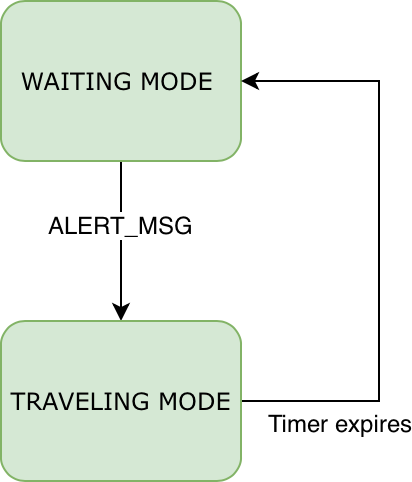
\includegraphics[width=0.35\textwidth]{resources/truck_state_chart}
	\caption{Truck FSM.}
	\label{fig:truck-fsm}
\end{figure}

\begin{figure}[H]
    \begin{minipage}[t]{0.55\textwidth}
        \centering
        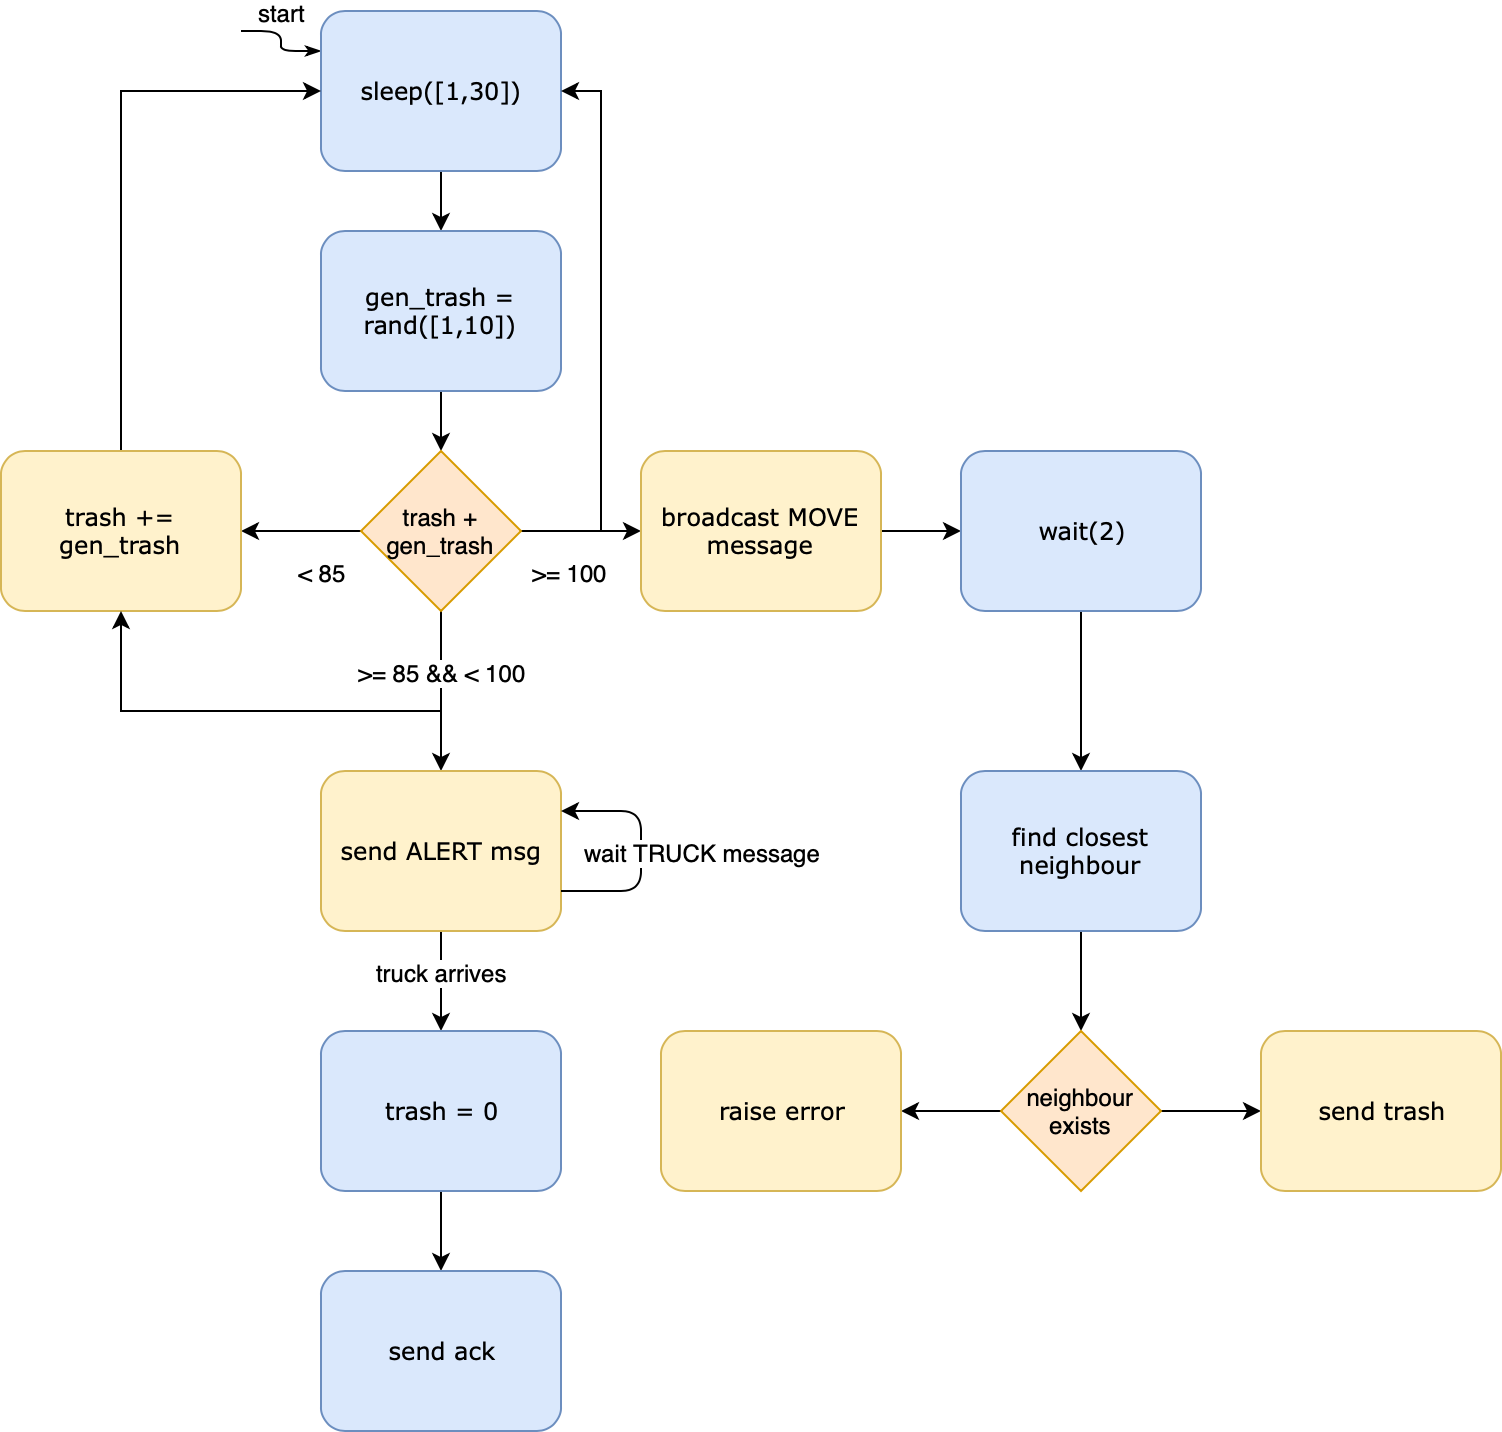
\includegraphics[width=1\textwidth]{resources/bin_flow_chart}
        \caption{Bin flowchart.}
        \label{fig:bin-flow}
    \end{minipage}
    \hspace*{\fill}
    \begin{minipage}[t]{0.37\textwidth}
        \centering
        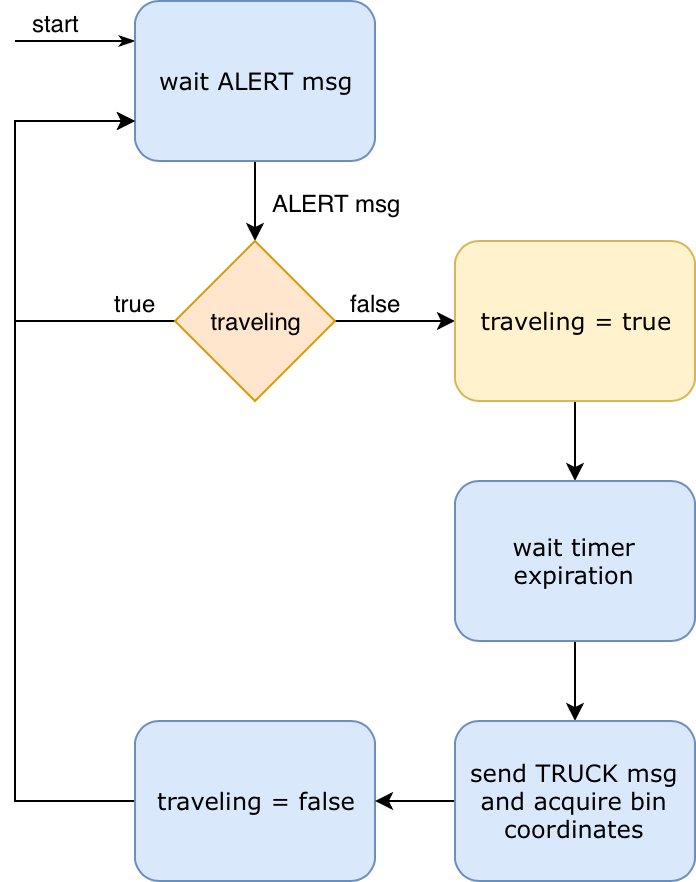
\includegraphics[width=1\textwidth]{resources/truck_flow_chart}
        \caption{Truck flowchart.}
        \label{fig:bin-flow}
    \end{minipage}
\end{figure}

\subsection{Bin firmware}

The bin firmware is composed of three main processes, one for each of the three operation modes:

\begin{itemize}
    \item \texttt{trash\_proc} -- handles the periodic generation of the trash;
    \item \texttt{alert\_mode\_proc} -- handles the period transmission of \texttt{ALERT} messages.
    \item \texttt{full\_mode\_proc} -- handles the neighbor mode, in particular the broadcast of the \texttt{MOVE} message, the selection of the closest bin and the transmission of the exceeding trash to it.
\end{itemize}

There actually is a fourth process in the firmware, used to reply to a \texttt{MOVE} message. We chose to place this routine in a separate process and not to leave it in the unicast callback in order not to lock the communication processes.

\subsection{Truck firmware}

The truck firmware is composed on a single process, which handles the traveling simulation (it sets up a timer and waits for its expiration) and the transmission of the \texttt{TRUCK} message.

\subsection{Other implementation details}

\begin{itemize}
	\item We adopted two different transmission methods, both of them part of the native Rime communication stack:
		\begin{itemize}
			\item \href{http://contiki.sourceforge.net/docs/2.6/a01720.html}{\textbf{Broadcast}} -- The broadcast module sends packets to all local area neighbors with an a header that identifies the sender. No retransmission and acknowledgement implemented.
			\item \href{http://contiki.sourceforge.net/docs/2.6/a01738.html}{\textbf{RUnicast}} -- The runicast primitive uses acknowledgements and retransmissions to ensure that the neighbor successfully receives the packet, thus we were able to avoid implementing an explicit acknowledgement system (e.g., the ACK sent by the bin upon setting its trash to 0).
		\end{itemize}
	\item The random coordinates generated by each node at startup are limited between 0 (inclusive) and 50 (exclusive).
	\item The time interval between two consecutive \texttt{ALERT} messages sent out by the same node is statically set to 10 seconds.
	\item $\alpha_\mathrm{bin-bin} = 0.01$ and $\alpha_\mathrm{truck-bin} = 0.75$
	\item For Node-RED dashboard we used two external plugins that have to be manually installed: \texttt{ui\_led}, \texttt{node-red-dashboard}.
\end{itemize}







\end{document}
